{\color{gray}\hrule}
\begin{center}
\section{Hasil dan Pembahasan}
\textbf{Hasil dapat berupa gambar hasil praktikum, maupun data hasil praktikum}
\end{center}
{\color{gray}\hrule}
\begin{enumerate}

\item \textbf {Menjalankan Ubuntu dan Instalasi Hadoop}: \\ \\
    	\colorbox{BurntOrange}{wget https://dlcdn.apache.org/hadoop/common/hadoop-3.3.6/hadoop-3.3.6.tar.gz} \\ \\
    	
    	
\item \textbf {Beralih ke user hdoop}: \\ \\
\colorbox{BurntOrange}{su - hdoop} \\ \\
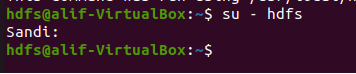
\includegraphics[scale=.6]{Gambar/satu} \\
    	
\item \textbf {Verifikasi Instalasi Java}: \\ \\
\colorbox{BurntOrange}{java -version} \\ \\
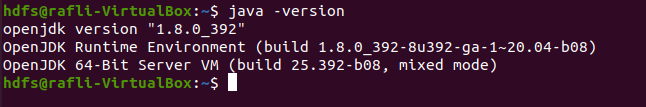
\includegraphics[scale=.6]{Gambar/dua} \\
    	
\item \textbf {Menjalankan Peintah-Perintah Hadoop}: \\ \\
\colorbox{BurntOrange}{start-dfs.sh} \\ \\
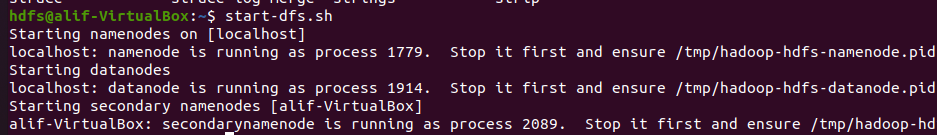
\includegraphics[scale=.5]{Gambar/tiga} \\
    	
\item \textbf {Verifikasi Hasil Instalasi Apache Spark}: \\ \\
\colorbox{BurntOrange}{pyspark --version} \\ \\
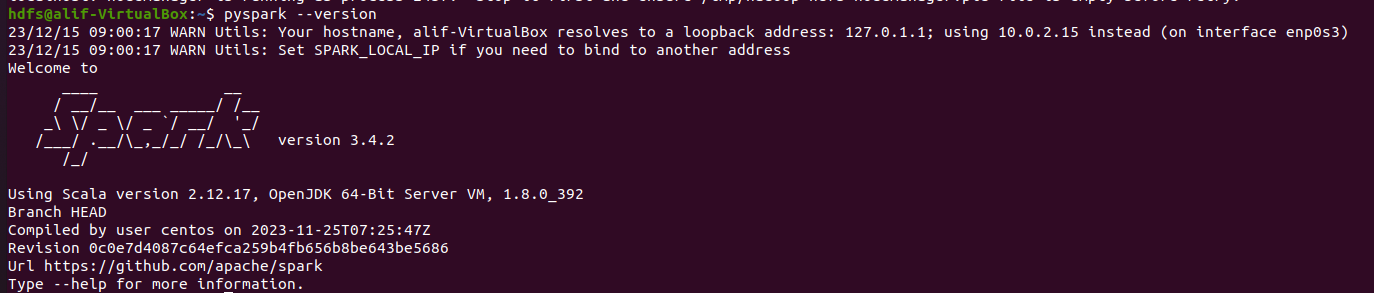
\includegraphics[scale=.4]{Gambar/empat} \\

\item \textbf {Menjalankan perintah jps}: \\ \\
\colorbox{BurntOrange}{jps} \\ \\
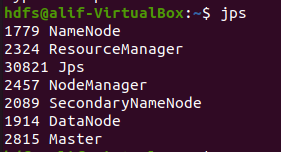
\includegraphics[scale=.4]{Gambar/lima} \\

\item \textbf {Menjalankan hadoop service di localhost}: \\ \\
\colorbox{BurntOrange}{Akses melalui web browser dengan alamat http://localhost: 98705 atau http://localhost:80886
.} \\ \\
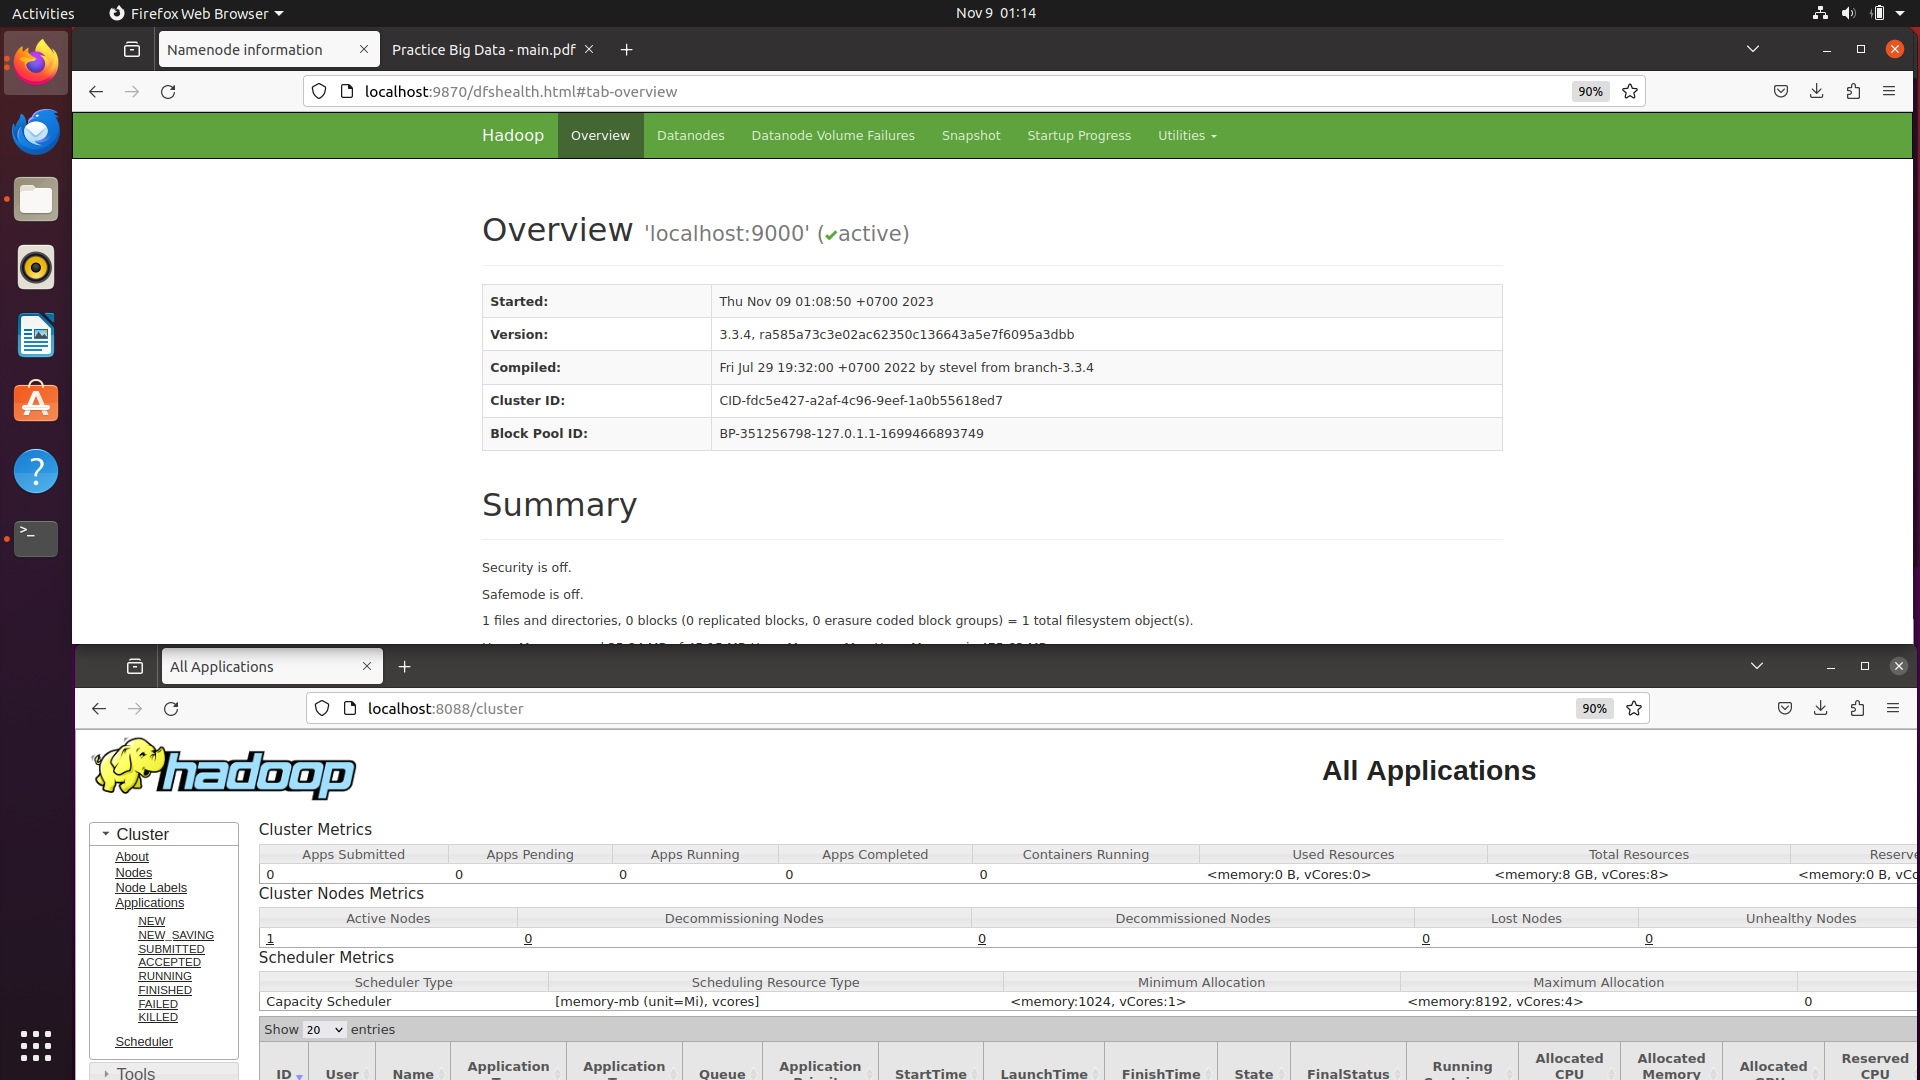
\includegraphics[scale=.2]{Gambar/hadoop sukses} \\

\item \textbf {Melihat hasil part 3}: \\ \\
\colorbox{BurntOrange}{hadoop fs -ls /output} \\ \\
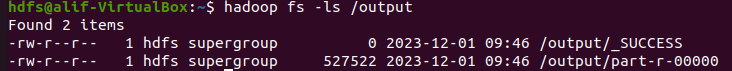
\includegraphics[scale=.4]{Gambar/enam} \\

\item \textbf {Melihat hasil grafik}: \\ \\
\colorbox{BurntOrange}{spark - submit MLPySpark.py} \\ \\
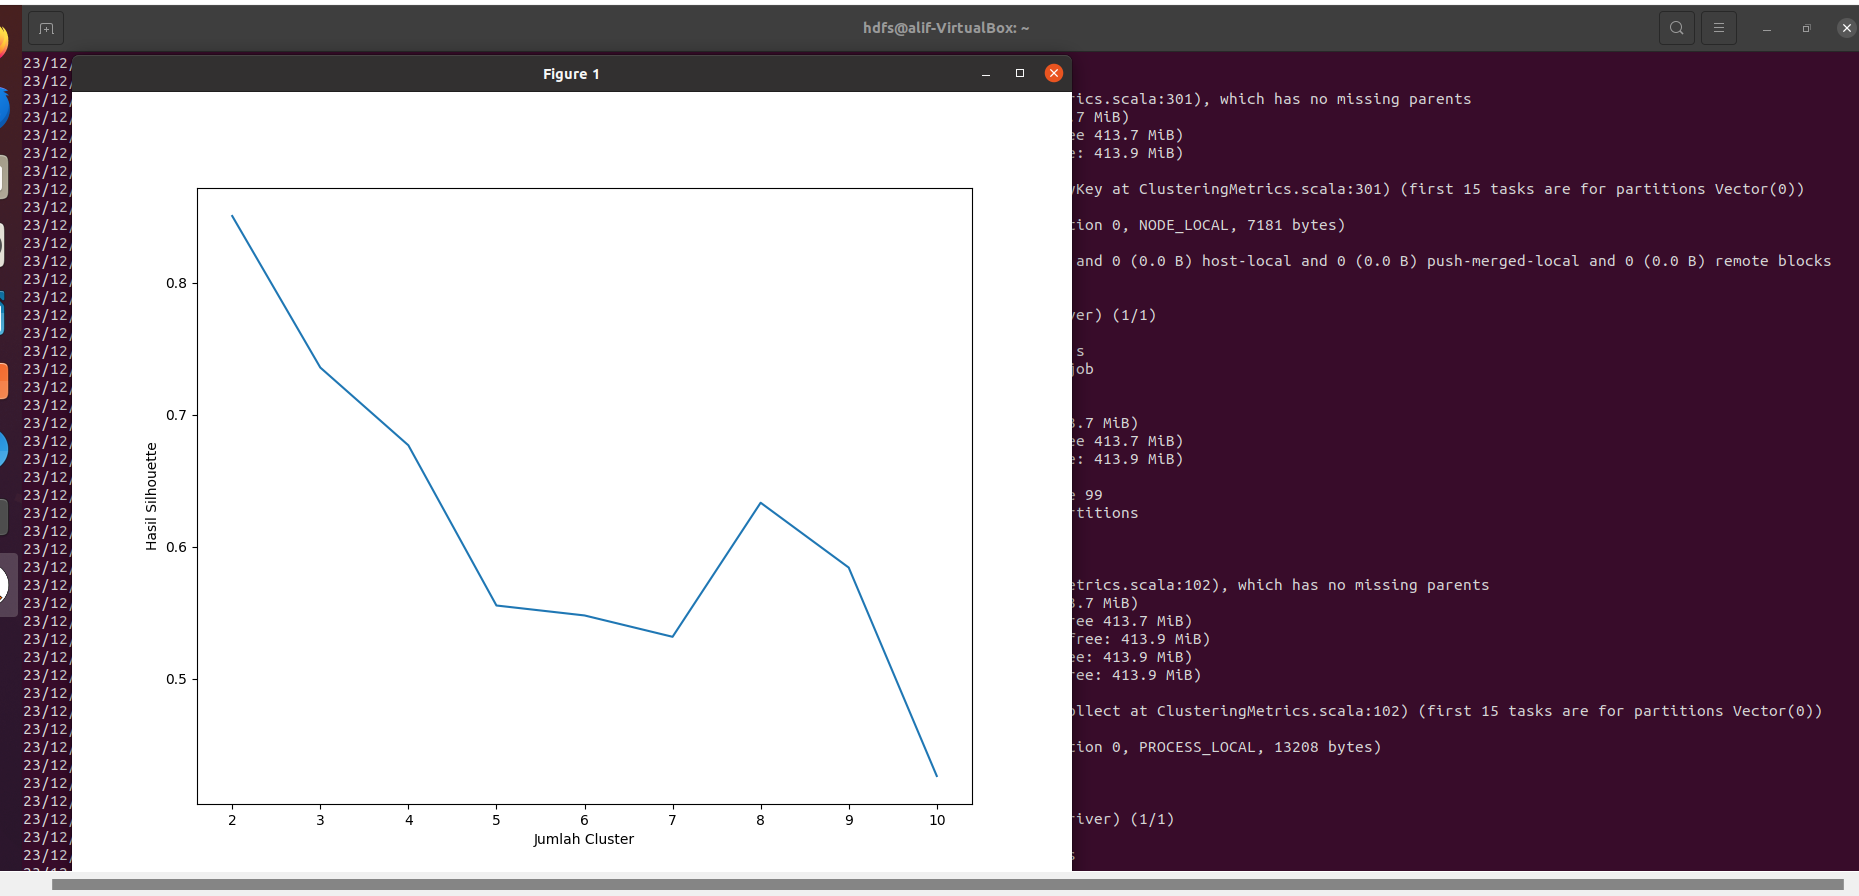
\includegraphics[scale=.4]{Gambar/tujuh} \\



    	
    	
 
    	
    	 	
    	
    	
    	
    	
    	
    	
    	
    	
    	
    	
    	
    	
    	
    	
    	
    	
    	
    	
    	
    	
    	
    	
    	
    	
    	
    	
    	
    	
    	
    	
    	
    	
    	
    	
    	
    	
    	
    	
    	
    	
    	
    	
    	
    	
    	
    	
    	
    	
    	
    	
    	
    	
    	
    	
    	
    	
    	
    	
    	
    	
    	
    	
    	
    	
    	
    	
    	
    	
    	
\end{enumerate}

